\section{Dilema prizonierului}

Dilema prizonierului\footnote{Adaptare după \textit{Prisoner's Dilemma: Game Theory}, Merrill M. Flood, Melvin Dresher, Albert W. Tucker, Framing Device, Experimental Economics} reprezintă o problemă tratată în teoria jocurilor.
\\
\\
TODO: UN PARAGRAF DESPRE IMPLICATII IN ALTE DOMENII \\
\\
A fost formulată în anul 1950 de către Merrill Flood și Melvin Dresher, angajați ai companiei RAND Corporation\footnote{https://www.rand.org/}. Denumirea- dilema prizonierului- este meritul lui Albert W. Tucker, de la Universitatea Princeton, care a formalizat jocul și a introdus noțiunea de răsplată (engl. payoff).
 
Enunțul clasic al problemei este prezentat în paragraful următor: 

\begin{quote} 
	\textit{Doi suspecți sunt arestați de către poliție. Polițiștii nu au suficiente dovezi pentru a condamna suspecții așa că îi duc în camere separate și le propun aceeași ofertă amândurora. Dacă unul dintre suspecți depune mărturie pentru urmărirea penală împotriva celuilalt suspect și celălalt tăinuiește faptele, cel care a trădat este eliberat și cel care a tăinuit primește o pedeapsă de 10 ani de închisoare. Dacă ambii suspecți nu mărturisesc, ambii ajung în pușcarie pentru jumătate de an. Dacă se trădează reciproc, fiecare primește o pedeapsă de 5 ani. Suspecții au de ales între a trăda și a tăinui faptele.}
\end{quote}

TODO: DE ADAUGAT UN DESEN CARE SA ILUSTREZE MAI CLAR MATRICEA RECOMPENSELOR, dupa modelul de mai jos \\

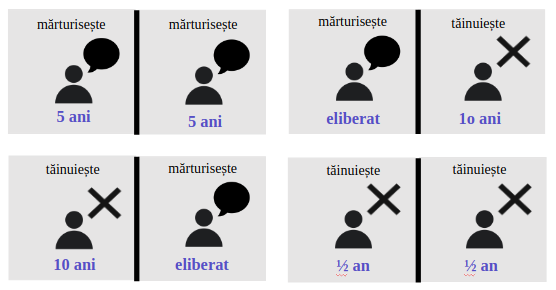
\includegraphics[
	width=10cm,
	height=6cm,
	keepaspectratio
]
{imagini/matrice.png}\\


Putem formaliza aceast paragraf prin următoarea matrice a recompenselor, unde cei doi suspecți sunt numiți \textbf{A} și \textbf{B}\footnote{Preluat din https://plato.stanford.edu/entries/prisoner-dilemma/}. Se prezintă rezultatele obținute pentru fiecare combinație dintre tăinuire și marturisire \footnote{Considerăm că atunci când un suspect mărturisește, mărturia să îl incriminează pe celălalt suspect.}:  

\begin{table}[H]
	\centering
	\def\arraystretch{1.75}
	\begin{tabular}{|c|c|c|c|}
		\hline
		\multicolumn{2}{|c|}{\textbf{Acţiune aleasă}} & \multicolumn{2}{c|}{\textbf{Rezultat obţinut}} \\ \hline
		\textbf{A} & \textbf{B} & \textbf{A} & \textbf{B} \\ \hline
		tăinuiește & tăinuiește & \textbf{Reward} & \textbf{Reward} \\ \hline
		tăinuiește & mărturiseşte & \textbf{Sucker's payoff} & \textbf{Temptation} \\ \hline
		mărturiseşte & tăinuiește & \textbf{Temptation} & \textbf{Sucker's payoff} \\ \hline
		mărturiseşte & mărturiseşte & \textbf{Punishment} & \textbf{Punishment} \\ \hline
	\end{tabular}
	\caption{\textit{Adaptare după matricea recompenselor pentru dilema prizonierului}}
	\label{matricea_recompenselor}
\end{table}

Termenii care apar în tabel sunt următorii: 
 
\begin{itemize} 
	\item \textbf{Temptation}: recompensa obținută de jucatorul ce mărturisește atunci când celalalt tăinuiește faptele 
	\item \textbf{Reward}: recompensa pentru când cei doi suspecți, A și B, aleg să tăinuiască 
	\item \textbf{Punishment}: pedeapsa obținută de fiecare dintre cei doi suspecți atunci când se trădează reciproc 
	\item \textbf{Sucker's payoff}: pedeapsa pentru cel care a tăinuit atunci când celălalt l-a trădat 
\end{itemize} 
 
Pentru a face trecerea de la pedeapsa cu închisoarea la ideea de joc, considerăm că cei 4 termeni reprezintă scoruri de valoare pozitivă și că scopul suspecților este să obțină un număr cât mai mare de puncte. 

Între acești termeni ce reprezintă recompensele, se respectă următorul lanț de inegalități: 

\begin{center} 
	\textbf{Temptation} \textgreater \textbf{Reward} \textgreater \textbf{Punishment} \textgreater \textbf{Sucker's payoff} 
\end{center} 

TODO: DE PUS INEGALITATEA INTR-O CASETA\\

\section{Strategii pentru dilema prizonierului}

Dacă suspectăm că celălalt reținut va tăinui faptele, suntem mai avantajați dacă mărturisim (vom fi "răsplătiți" cu \textbf{Temptation}, despre care știm că are o valoare mai mare decât \textbf{Sucker's payoff}- scorul pe care îl va obține celălalt suspect), decât dacă tainuim (caz în care toți primesc \textbf{Reward}; \textbf{Temptation} \textgreater \textbf{Reward}).

Dacă suspectăm că celălalt va mărturisi împotriva noastră, suntem mai avantajați dacă mărturisim și noi (vom primi amândoi \textbf{Punishment}), decât dacă tainuim (caz în care primim \textbf{Sucker's payoff}, însă celalt va primi un scor mai bun, \textbf{Temptation}).

În alte cuvinte, indiferent de mișcarea celuilalt jucător, \textbf{strategia care ne avantajează câștigul personal, în defavoarea câștigului celuilalt jucător, este mărturisirea împotriva acestuia}.

Dilema este dată de faptul că ambii suspecți ar fi obținut un scor mult mai bun dacă ar fi tăinuit amândoi (protejând pe celălalt participant), decât dacă amândoi ar fi ales să mărturisească (în defavoarea celuilalt suspect). Pe scurt, cooperarea celor doi aduce cel mai mare avantaj de ambele părți.

\section {Problema iterată a prizonierului} 

Dacă s-ar juca mai multe runde, în care ambii jucători ar alege să se trădeze reciproc la fiecare rundă, scorul pe care l-ar obține ar fi mult mai mic decât dacă ar alege să tainuiasca faptele în fiecare rundă. 

În teoria jocurilor, problema iterată a prizonierului este catalogat drept joc cu suma nenulă \footnote{Numim joc de sumă nenulă jocul în care suma câstigurilor este diferită de zero.} (engl. non-zero-sum game).

Un meci între doi jucători este reprezentat de un număr de runde, care nu este cunoscut de catre participanți.

În fiecare rundă, cei doi jucatarori aleg independent, în secret, ce mișcare vor face: vor tăinui sau vor mărturisi. La final de rundă, cei doi își expun alegerea. În funcție de ce mișcare au ales cei doi, fiecare este răsplătit cu un anumit câștig, care se adaugă la scorul total individual al jucătorilor. 

Dacă la o anumită rundă ambii au cooperat, scorul ambilor jucători va crește cu o valoare ce poartă denumirea de \textbf{Reward}. 

Dacă ambii trădează, vor primi \textbf{Punishment payoff}. 

Dacă unul cooperează, dar celălalt trădează, cel care a cooperat primește \textbf{Sucker's payoff} și celălalt este răsplătit cu \textbf{Temptation}. 

\section {Strategii pentru problema iterată a prizonierului}

Considerând acest scenariu drept un joc, folosim termenul de \textbf{cooperare} (engl. cooperation) pentru a descrie situația când unul dintre suspecți \textbf{tăinuiește} faptele. \textbf{Mărturisirea} faptelor de către un suspect pentru incriminarea celuilalt suspect va fi numită \textbf{trădare} (engl. defection). 

\subsection{Turneele lui Axelrod}

Printre studiile pofesorului Robert Axelrod, care predă științe politice și politici publice la Universitatea din Michigan, se află și problema iterată a prizonierului.

Interesul său de a afla o strategie potrivită l-a determinat să organizeze două turnee de tip \textit{fiecare cu fiecare} (engl. round-robin). În aceste turnee, fiecare participant joacă pe rând împotriva tuturor celorlalți \footnote{https://dictionary.cambridge.org/dictionary/english/round-robin}.  Primul turneu a inclus 14 programe ce furnizează strategii de joc, iar cel de al doilea a avut un număr de 63 de programe.

Observațiile sale sunt trecute în lucrarea \textit{The Evolution of Cooperation}, scrisă în 1984\footnote{Adaptare după \textit{Genetic Algorithms: An Overview}, Melanie Mitchell, 1995.}.

Axelrod a solicitat participanților strategii sub formă unor programe care cunosc istoricul ultimelor trei runde.

Câștigătorul ambelor turnee a fost strategia \textbf{Tit-for-Tat}. Această strategie cooperează la prima rundă, apoi, în următoarele runde, utilizează mișcarea făcută de oponent în runda anterioară. În alte formă de idei, cooperează de fiecare dată când celălalt cooperează și trădează când este trădată, dar nu inițiază trădarea.

\subsection{Strategii analizate}

În următoarele rânduri, sunt enumerate câteva strategii analizate:

\begin{itemize}  
	\item \textbf{Always cooperate}: Jucătorul cooperează la fiecare rundă a jocului, indiferent de strategia aplicată de celălalt jucător. 
	\item \textbf{Always defect}: Jucătorul trădează la fiecare rundă a jocului. 
	\item \textbf{Grudger}: Această strategie presupune cooperarea la fiecare rundă, până la prima trădare din partea celuilalt jucător. Așadar, adoptând această strategie, dacă oponentul trădează chiar și o singură dată, următoarele mișcări, până la final de joc, vor fi de trădare. 
	\item \textbf{Pavlov}: Se alege cooperarea la prima rundă. Dacă la runda anterioară jucătorul a fost recompensat cu \textbf{Temptation}\footnote{\textbf{Temptation} este recompensa obținută de jucatorul ce trădează atunci când oponentul cooperează.} sau \textbf{Reward}\footnote{\textbf{Reward} reprezintă recompensa primită de ambii jucători atunci când cooperează.}, acesta repetă ultima mișcare. În celălalt caz, alege mișcarea opusă. 
	\item \textbf{Random}: Se alege la întâmplare următoarea acțiune. 
	\item \textbf{Tit-For-Tat}: Se alege cooperarea la prima rundă. De la runda a doua, jocuatorul ce alege această strategie repetă ultima mișcare a oponentului. 
	\item \textbf{Suspicious Tit-For-Tat}: Diferența dintre această strategie și \textbf{Tit-For-Tat} este că la prima mișcare se alege trădarea. 
	\item \textbf{Tit-For-Two-Tats}:  Jucătorul cooperează de fiecare dată, făcând excepție acele cazuri în care jucătorul este trădat de două ori consecutiv. 
\end{itemize}  

